\documentclass[11pt,letterpaper]{ctexart}
\usepackage[margin=0.82in]{geometry}
\usepackage{booktabs,longtable,array}
\usepackage{graphicx}
\usepackage{caption}
\usepackage{hyperref}
\usepackage{xcolor}
\usepackage{float}
\setCJKmainfont{Noto Serif CJK SC}
\setlength{\parskip}{3pt}
\setlength{\parindent}{2em}
\captionsetup{font=small,labelfont=bf}
\hypersetup{colorlinks=true,linkcolor=black,urlcolor=blue,pdftitle={FewClick Supplementary Material},pdfauthor={Anonymous}}
\graphicspath{{额外可视化/}{额外可视化/TLS30_review_panels/}}
\newcommand{\code}[1]{\texttt{#1}}
\begin{document}

\begin{center}
{\LARGE \textbf{FewClick：可复现性技术附录}}\\[5pt]
{\large 匿名投稿补充材料（中文工作稿）}
\end{center}

\noindent\textbf{说明。} 本文档是论文 \emph{A Few-Click Interactive Framework for User-Specified Histopathological Tissue Segmentation} 的独立技术附录。所有训练、验证和外部评估均使用在相应阶段冻结的配置；本文件不包含作者、机构、绝对数据路径、医院名称或原始病例标识。可执行代码、匿名化配置和使用说明另以 \code{code\_and\_data.zip} 作为代码与数据附件提供。

\section{数据集与数据划分}
\subsection{主开发队列}
主实验使用 200 张 H\&E 全切片图像（WSI）构成的组织分割开发队列。像素级标注包括 12 个组织类别：肿瘤上皮、肿瘤间质、背景、坏死、正常腺体、正常间质、黏膜下层/浆膜、肌肉、淋巴细胞聚集、黏液、脂肪和血液。背景标签不作为前景目标，忽略标签为 255。

划分在 WSI 层面完成，以患者/WSI 标识为分组键：140 张训练、30 张验证、30 张独立测试；同一 WSI 的图像区域不跨集合。测试集在模型结构、超参数和阈值冻结前不参与模型选择或消融。所有图像在 10$\times$ 目标倍率下建立索引，图像块为 $512\times512$ 像素、步长为 512；仅使用有效像素比例不少于 0.50 且组织比例不少于 0.30 的候选块。

训练样本按类别内部/类别边界/稀有类别/背景或困难负例以 0.30/0.30/0.30/0.10 混合。稀有类别的训练占比上限为 0.02，边界块阈值为 0.02。

\subsection{外部 TLS 队列}
额外泛化实验使用与主开发队列完全隔离的 30 张 H\&E WSI，目标为训练标签中未出现的三级淋巴结构（TLS）。该队列不参与训练、验证、检查点选择或超参数调整。模型参数在此实验中完全冻结。

30 张 WSI 共包含 578 个 TLS 多边形；其中 279 个多边形提供正提示，299 个完全留出，用于测量由局部提示驱动的远距离 TLS 检索。每张 WSI 的提示与留出划分在推理前固定。

\section{提示采样与评估协议}
\subsection{主实验的 episodic 提示}
一个 episode 包含 WSI 图像区域、目标组织类别、对应二值掩膜、正提示集合和可选负提示集合。每个训练 epoch 使用 20,000 个 episode；固定验证清单包含 4,000 个 episode。除被移除的目标模块外，消融变体共享数据划分、随机种子、提示清单、数据增强和优化计划。

提示大小按点/小区域/大区域以 0.40/0.35/0.25 采样；位置按类别内部/类别边界/稀有类别/背景或困难负例以 0.30/0.30/0.30/0.10 采样。困难负例来自相邻组织、特征空间近邻及模型的高置信误检区域。主实验采用 $(1+1)$、$(3+1)$ 和 $(5+1)$ 三种交互预算，分别为 1、3、5 个正点加 1 个负点。

全切片主实验的每个 WSI--组织任务使用 1 个正点和 1 个负点。推理前冻结 5 组提示，以与结果无关的均值$\pm$标准差汇总；若正负提示被映射到同一硬区域，则该次提示冲突按空预测计分，不使用 GT 重新选择候选。

\subsection{外部 TLS 的提示与检索评估}
每张外部 WSI 中，约一半的 TLS 多边形各提供 1 个正提示；从未标注 TLS 的组织区域采样 3 个负提示。其余 TLS 多边形完全不参与提示，并作为留出检索目标。推理采用 10$\times$ 坐标系，切块大小为 512、步长为 384，level-0 至评估坐标的下采样因子为 4。

主要报告两类指标：(i)~\textbf{未提示多边形召回率}，即未参与提示的 TLS 是否被检索到；(ii)~\textbf{去提示区指标}，即将已提示 TLS 像素从评估域中剔除后计算 Dice、精确率和召回率。单一多边形的精确率/Dice 不作为整体质量主指标，因为同张 WSI 中其他 TLS 的正确预测会被该口径误记为假阳性。

\section{训练配置与模型选择}
所有随机过程使用配置文件记录的种子：Phase 1/2 使用 20260714，Phase 3 使用 20260719，Phase 5/6 及 TLS 推理使用 20260720。推理的二值阈值固定为 0.5。

\footnotesize\sloppy
\begin{longtable}{p{0.13\linewidth}p{0.25\linewidth}p{0.27\linewidth}p{0.25\linewidth}}
\caption{各训练阶段的最终配置。}\label{tab:hyperparameters}\\
\toprule
阶段 & 模型与结构 & 训练设置 & 优化与损失\\
\midrule
\endfirsthead
\toprule
阶段 & 模型与结构 & 训练设置 & 优化与损失\\
\midrule
\endhead
Phase 1：10$\times$视觉特征 & DeepLabV3--ResNet50；12 类；$512\times512$ 输入 & 30 epochs；每 GPU batch 8；每 epoch 20,000 样本；验证 4,000；2 workers/GPU；AMP；梯度累积 1；warm-up 2 epochs & LR $10^{-4}$；weight decay $10^{-4}$；交叉熵/Dice 权重 0.5/1.0\\
Phase 2：可学习区域 & 64 个区域；维度 256；空间温度 0.08；由 Phase 1 检查点初始化 & 30 epochs；batch 8/GPU；20,000/4,000 训练/验证样本；bf16 AMP；SLIC 保持 5 epochs、衰减 15 epochs & 主干/区域头 LR $10^{-5}/10^{-3}$；weight decay $10^{-4}$；梯度裁剪 5.0；SLIC/边界/均衡/紧致/纯度/语义 CE/语义 Dice 权重为 1.0/1.0/0.50/0.10/0.25/0.50/1.0\\
Phase 3：细胞感知区域表示 & 每块最多 255 个细胞；细胞特征维度 74；64 个区域、维度 256；冻结 Phase 2 & 30 epochs；batch 4/GPU；20,000/4,000；bf16 AMP & LR $10^{-3}$；weight decay $10^{-4}$；梯度裁剪 5.0\\
Phase 4：跨尺度交互 & 冻结 Phase 2/3；10$\times$/5$\times$/2.5$\times$ 各 64 个 256 维 token；1 个层级图块；每子节点保留 top-4 物理重叠父节点 & 30 epochs；batch 16/GPU；20,000/4,000；bf16 AMP & AdamW；LR $10^{-3}$；weight decay $10^{-4}$；梯度裁剪 5.0；12 类区域交叉熵（忽略标签 255）\\
Phase 5：提示集合编码 & 区域维度 256；4 heads；2 个 set-encoder 层；dropout 0.10 & 30 epochs；batch 32/GPU；20,000/4,000；bf16 AMP & LR $10^{-3}$；weight decay $10^{-4}$；梯度裁剪 5.0；Dice/ranking 权重 1.0/0.2；margin 0.2\\
Phase 6：最终联合模型（J5） & 区域维度 256；图 heads 4；图层 2；每节点 6 邻居；dropout 0.10；KNN=4；仅解冻 backbone layer 4 & 5 epochs；batch 2/GPU；20,000/4,000；bf16 AMP & layer-4 LR $10^{-6}$；其余预设 LR：parent-context/decoder/prompt/Phase-2 embedding/assignment 为 $10^{-4}/10^{-4}/10^{-5}/5\times10^{-6}/2\times10^{-5}$；weight decay $10^{-4}$；梯度裁剪 5.0\\
\bottomrule
\end{longtable}
\fussy\normalsize

\section{硬件与软件环境}
实验使用 Linux 与 conda 环境 \code{aligner}。主训练和全切片批处理均使用多 GPU；外部 TLS 批量推理使用 6 张 GPU（逻辑编号 0--5），每张 GPU 的推理 batch size 为 2、数据加载 workers 为 4。细胞特征提取使用单 GPU，XCellFormer batch size 为 8、Cellpose 网络 batch size 为 8。线程设置为 \code{OMP\_NUM\_THREADS=8}、\code{MKL\_NUM\_THREADS=8}、\code{OPENBLAS\_NUM\_THREADS=8}、\code{NUMEXPR\_NUM\_THREADS=8} 和 \code{VIPS\_CONCURRENCY=4}。

\begin{center}\small
\begin{tabular}{ll}
\toprule
项目 & 版本/配置\\ \midrule
GPU & 6 $\times$ NVIDIA RTX 5880 Ada Generation，单卡 49,140 MiB（约 48 GiB）\\
NVIDIA 驱动 / 系统 CUDA & 550.67 / 12.4\\
操作系统 & Linux\\
Python & 3.10.19\\
PyTorch & 2.9.1+cu128\\
CUDA runtime & 12.8\\
NumPy & 2.2.6\\
pandas & 2.3.3\\
PyYAML & 6.0.3\\
Cellpose & 4.0.7\\
OpenSlide & 4.0.0（\code{openslide-python} 1.4.2）\\
pyvips / libvips & 2.2.3 / 8.16.0\\
\bottomrule
\end{tabular}
\end{center}

\section{额外定量结果：30 张外部 TLS WSI}
结果来自固化的 30/30 完整批处理。所有数值由冻结模型在未参与开发的外部数据上得到。

\begin{center}\small
\begin{tabular}{lr}
\toprule
按 WSI 宏平均（每张 WSI 等权，均值 $\pm$ 标准差） & 值\\ \midrule
TLS 全部并集 Dice & $0.5229\pm0.2270$\\
TLS 全部并集精确率 & $0.4484\pm0.2554$\\
TLS 全部并集召回率 & $0.7882\pm0.0836$\\
未提示 TLS、去提示区 Dice & $0.3955\pm0.2319$\\
未提示 TLS、去提示区精确率 & $0.3139\pm0.2385$\\
未提示 TLS、去提示区召回率 & $0.7675\pm0.1373$\\
提示 TLS 多边形宏召回率 & $0.7274\pm0.1083$\\
\textbf{未提示 TLS 多边形宏召回率} & \textbf{$0.6968\pm0.1479$}\\
未提示多边形召回率 $\geq0.1$ 的比例 & $0.9416\pm0.1278$\\
未提示多边形召回率 $\geq0.5$ 的比例 & $0.7731\pm0.2078$\\
\bottomrule
\end{tabular}
\end{center}

\begin{center}\small
\begin{tabular}{p{0.45\linewidth}p{0.30\linewidth}r}
\toprule
统计口径 & 指标 & 值\\ \midrule
299 个未提示 TLS 多边形等权 & 宏召回率 & 0.6914\\
299 个未提示 TLS 多边形等权 & 召回率 $\geq0.1$ / $\geq0.5$ 的比例 & 0.9398 / 0.7559\\
299 个未提示 TLS 多边形按面积加权 & 召回率 & 0.7739\\
30 张 WSI 像素池化，TLS 全部并集 & Dice / 精确率 / 召回率 & 0.2785 / 0.1696 / 0.7785\\
30 张 WSI 像素池化，未提示 TLS 去提示区 & Dice / 精确率 / 召回率 & 0.1719 / 0.0967 / 0.7739\\
\bottomrule
\end{tabular}
\end{center}

单多边形的精确率和 Dice 会把同一 WSI 的其他 TLS 预测记为假阳性，因此不作为总体分割质量主指标。外部泛化主要依据未提示多边形宏召回率及去提示区域的 WSI 宏平均；像素池化反映大面积切片对全局计数的主导，不能与 WSI 宏平均混用。

\paragraph{未见数据与未见组织概念上的泛化。}
TLS 队列与主开发队列完全隔离，TLS 也不属于训练时的 12 个组织标签；推理过程中不进行任何参数更新、阈值校准或针对外部队列的提示优化。因此，这一实验要求模型仅从少量局部空间提示中推断当前的组织概念，并在整张切片中检索形态和组织学语义一致、但空间上与提示区域分离的 TLS。尽管没有见过该数据来源或 TLS 这一目标组织，冻结模型在 30/30 张 WSI 上均完成推理与评估；按 WSI 等权汇总，未提示 TLS 多边形的宏召回率为 $0.6968\pm0.1479$，去除已提示 TLS 区域后的召回率仍为 $0.7675\pm0.1373$。这表明模型的响应并不局限于点击周围的连通区域，而能够将局部提示转化为全切片范围的组织检索线索。

从更细粒度的留出多边形口径看，299 个未提示 TLS 中有 93.98\% 的多边形达到至少 0.1 的召回率，75.59\% 达到至少 0.5 的召回率；面积加权召回率为 0.7739。较高的召回覆盖说明，对大多数未参与提示的 TLS，模型能够提供可用于后续交互校正的候选区域。与此同时，Dice 和精确率受外部染色、组织背景差异及切片中大范围候选区域的影响较大；因此本实验应被解读为对\emph{未见组织概念的少样本跨数据集检索能力}的支持，而非对完全开放世界、无需交互的 TLS 分割性能的宣称。

\section{额外可视化}
\begin{figure}[H]
\centering
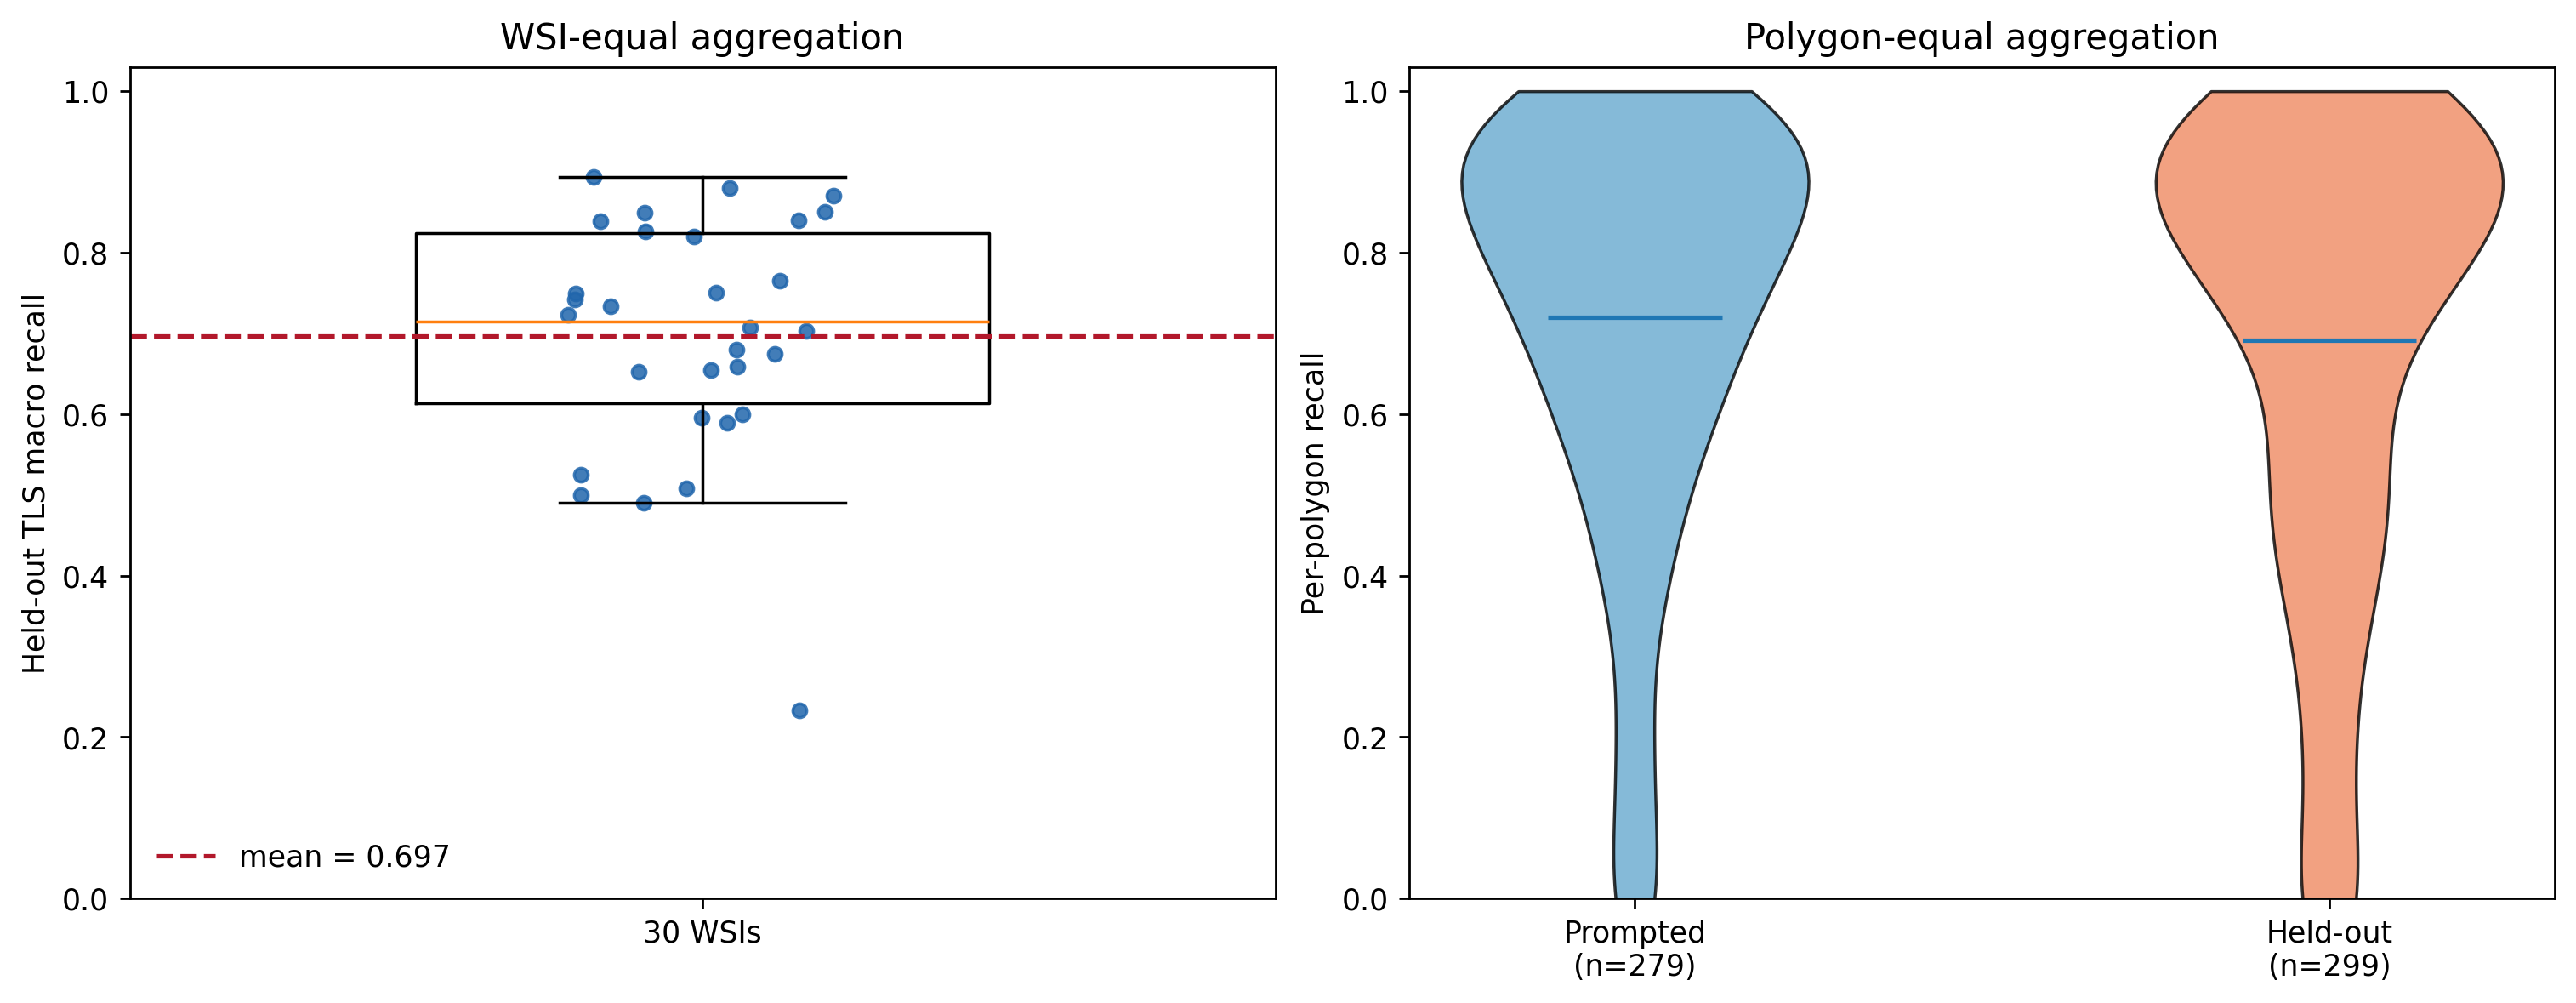
\includegraphics[width=\linewidth]{TLS30_retrieval_recall_distributions.png}
\caption{外部 TLS 检索的召回率分布。左：30 张 WSI 等权的未提示 TLS 宏召回率；右：提示（$n=279$）与留出（$n=299$）TLS 多边形等权召回率。两图的统计单位不同。}
\label{fig:tls-distribution}
\end{figure}

\begin{figure}[H]
\centering
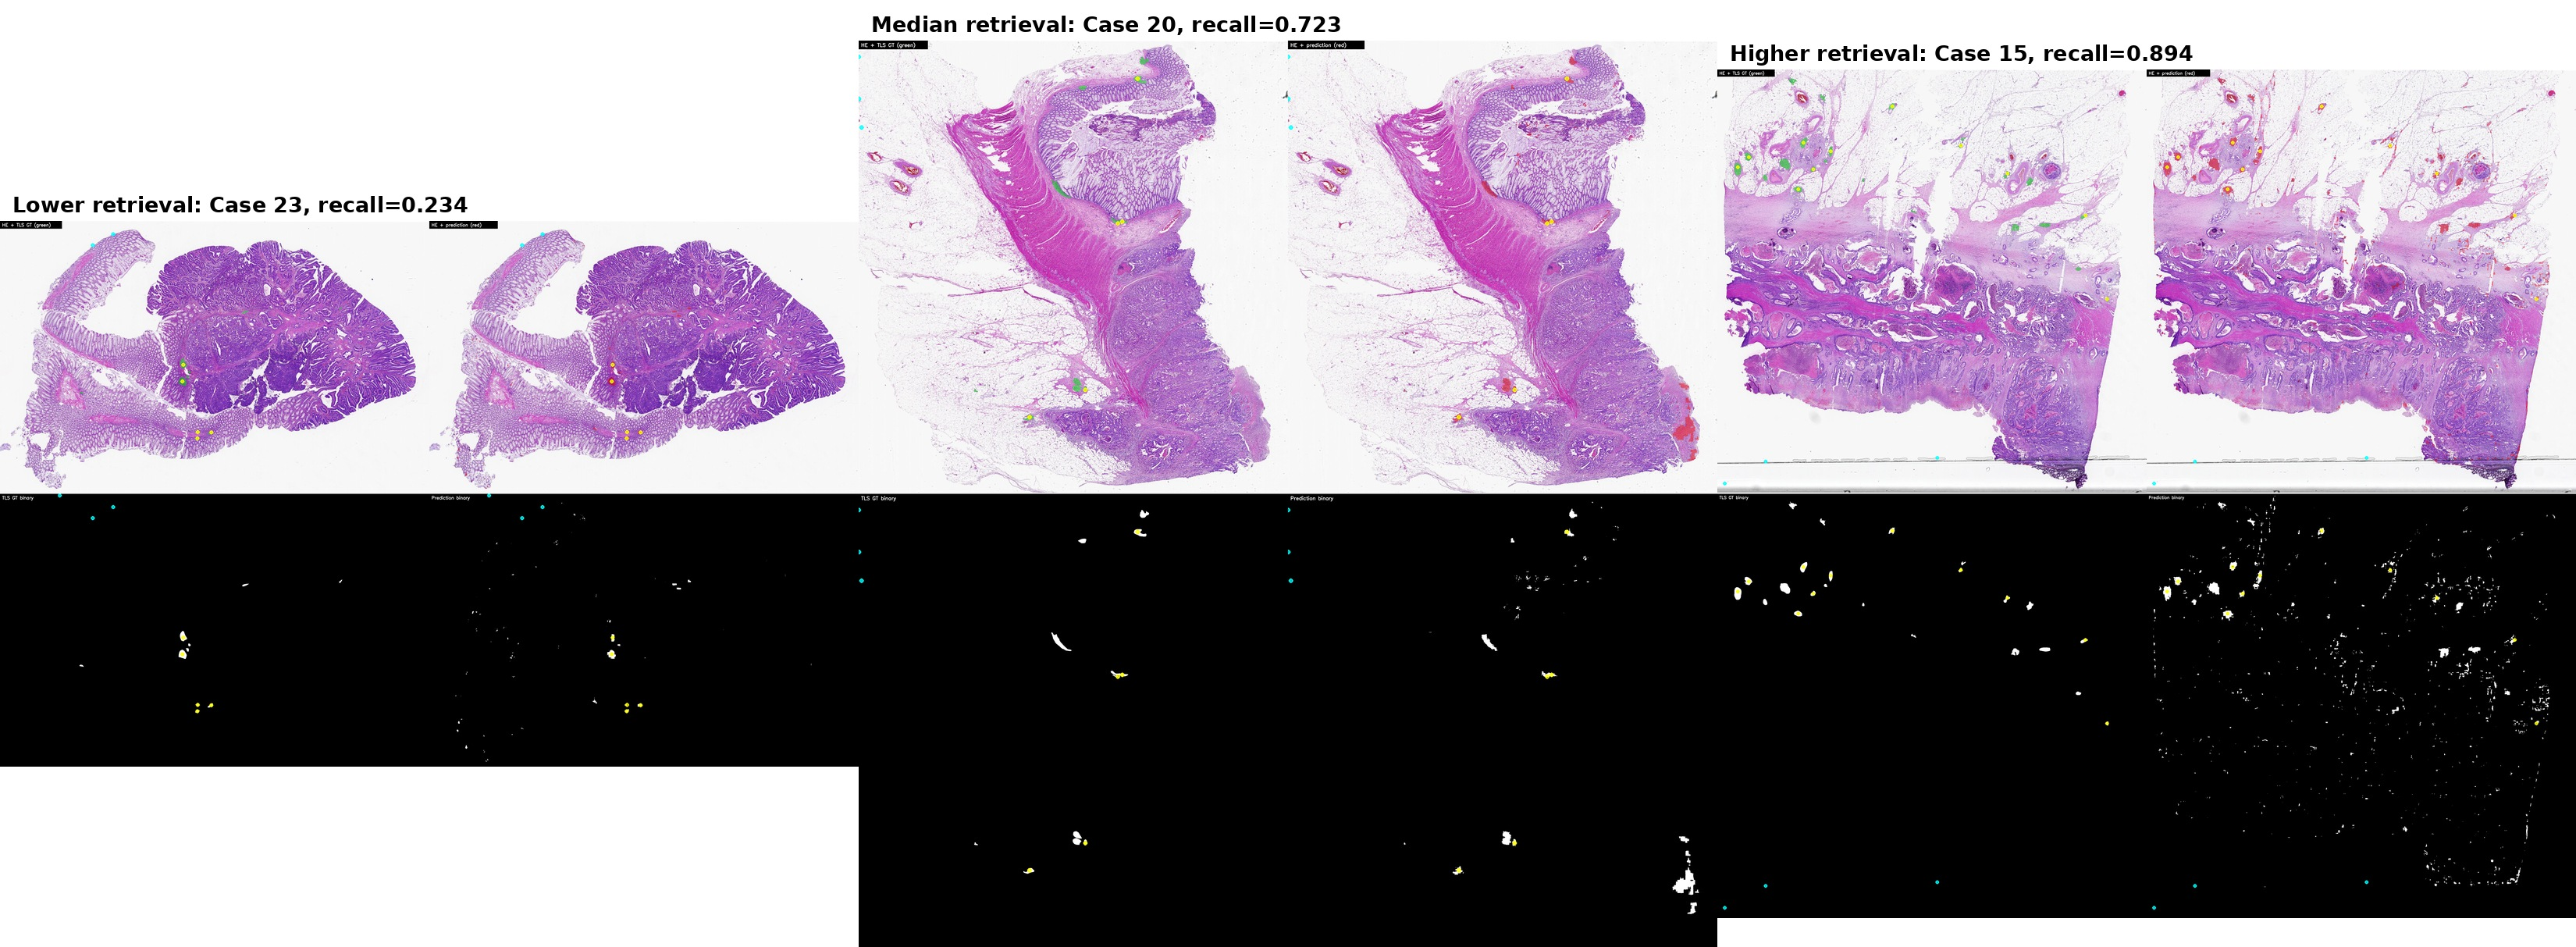
\includegraphics[width=0.97\linewidth]{TLS30_representative_retrieval_cases.jpg}
\caption{按未提示 TLS 宏召回率自动选择的低、中、高检索代表案例。每个四联图依次包含 H\&E+TLS GT、H\&E+预测、TLS GT 二值图和预测二值图。Case 编号仅表示预先固定的匿名清单顺序。}
\label{fig:tls-representatives}
\end{figure}

\section{可复现执行入口}
代码包中的核心入口按以下顺序组织：\code{data\_preprocess/} 生成组织/细胞配对与清单；\code{phase\_1\_multiscale/} 至 \code{phase\_6\_mask\_decoder/} 对应六个训练模块；\code{whole\_slide\_inference/} 执行冻结模型的 WSI 推理；\code{test\_TLS/} 提供外部 TLS 的病例准备、细胞特征提取、批量推理和检索评估。所有运行命令、参数和结果字段均在相应 README 与 YAML 配置中给出。

为保护匿名性，复现实验时应将受限数据和检查点放置在用户自有的本地位置，并通过命令行参数或相对路径配置替换。

\end{document}
